\documentclass[nogin, 10pt]{article}
\usepackage{natbib}
\usepackage[english]{babel}
\usepackage[latin1]{inputenc}
\usepackage[colorlinks = true]{hyperref}
\usepackage{bbm, amssymb, amsmath, amsthm}
\usepackage[T1]{fontenc} 
\usepackage{aeguill, fancyhdr, latexsym, mathrsfs, verbatim, colortbl}
\usepackage[a4paper,
            inner=30mm,
            outer=40mm,
            top=40mm,
            bottom=40mm,
            marginparwidth=30mm,
            marginparsep=5mm]{geometry}
\usepackage{tikz}
\usepackage{Sweave}


\setlength{\parindent}{0pt}
\setlength{\parskip}{1.3ex}

\begin{document}
\section{Regression}
\subsection{Maximum Likelihood Solution}
First we load the dataset, give it reasonable column names, and split it up into a training and a testing subset.
\begin{Schunk}
\begin{Sinput}
> rm(list=ls())
> setwd('~/github/StatML/Assignment2')
> load('./Data/bodyfat.RData')
> require(MASS)
> colnames(data)<-c('density','bodyFatPercentage','Age','Weight',
+                   'Height','Neck','Chest','Abdomen','Hip','Thigh',
+                   'Knee','Ankle','Biceps','Forearm','Wrist')
> ridx <- sample( 1:dim( data )[1], dim( data )[1] )
> trainIdx<-ridx[1:200]
> testIdx<-ridx[201:length( ridx )]
> train <- data[trainIdx,]
> test <- data[testIdx,]
\end{Sinput}
\end{Schunk}
We attempt to predict body fat using two models. The first one is based on weight, and chest, abdomen, and hip circumferences, and the second is based solely on abdominal circumference.
\begin{Schunk}
\begin{Sinput}
> selection1Train<-train[,c(4,7,8,9)]
> selection2Train<-train[,8]
> selection1Test<-test[,c(4,7,8,9)]
> selection2Test<-test[,8]
> targetTrain<-train[,2]
> targetTest<-test[,2]
\end{Sinput}
\end{Schunk}
We make a design matrix for every selection, and then find $\bf{w}_{\text{ML}}$ by $\bf{w}_{\text{ML}}=(\bf{\Phi}^{\text{T}}\bf{\Phi})^{-1}\bf{\Phi}^{\text{T}}\bf{t}$ where $(\bf{\Phi}^{\text{T}}\bf{\Phi})^{-1}\bf{\Phi}^{\text{T}}$ is the pseudo-inverse of $\bf{\Phi}$.
\begin{Schunk}
\begin{Sinput}
> design1Train<-as.matrix(cbind(seq(1,1,length.out=nrow(selection1Train)),
+                          selection1Train))
> design2Train<-as.matrix(cbind(1,selection2Train))
> wML1<-ginv(design1Train)%*%targetTrain
> wML2<-ginv(design2Train)%*%targetTrain
\end{Sinput}
\end{Schunk}
Once e have found $\bf{w}_{ML}$ we can apply it to the test set, via $y(\bf{x},\bf{w})=\bf{w}^{\bf{T}}\phi(\bf{x})$, and we can calculate the RMS via \[
\text{RMS}=\sqrt{\frac{1}{N}=\sum^N_{n=1}{(t_n-y(\bf{x}_n,\bf{w}))^2}}
\]

\begin{Schunk}
\begin{Sinput}
> design1Test<-as.matrix(cbind(seq(1,1,length.out=nrow(selection1Test)),
+                          selection1Test))
> design2Test<-as.matrix(cbind(seq(1,1,length.out=length(selection2Test)),
+                          selection2Test))
> y1<-t(wML1)%*%t(design1Test)
> y2<-t(wML2)%*%t(design2Test)
> RMS1<-sqrt(sum((targetTest-y1)^2)/length(targetTest))
> RMS2<-sqrt(sum((targetTest-y2)^2)/length(targetTest))
> print(RMS1)
\end{Sinput}
\begin{Soutput}
[1] 4.515678
\end{Soutput}
\begin{Sinput}
> print(RMS2)
\end{Sinput}
\begin{Soutput}
[1] 5.279117
\end{Soutput}
\end{Schunk}
Thus we get an RMS of 4.07 using the first model, and an RMS of 4.4 for the second model, showing the first model providing more accurate predictions. 

\begin{Schunk}
\begin{Sinput}
> y1Train<-t(wML1)%*%t(design1Train)
> y2Train<-t(wML2)%*%t(design2Train)
> RMS1Train<-sqrt(sum((targetTrain-y1Train)^2)/length(targetTrain))
> RMS2Train<-sqrt(sum((targetTrain-y2Train)^2)/length(targetTrain))
> print(RMS1Train)
\end{Sinput}
\begin{Soutput}
[1] 4.457727
\end{Soutput}
\begin{Sinput}
> print(RMS2Train)
\end{Sinput}
\begin{Soutput}
[1] 4.813506
\end{Soutput}
\end{Schunk}
For posterity, we have also calculated the error on the training set. For the two models, we get RMS of 4.52, and 4.81. The fact that the using the train error is not smaller than the test error, likely points to the fact that we are not over-fitting.

\subsection{Maximum a posteriori Solution}
In order to evaluat how different values of $\alpha$ influence our prediction, we vary $\alpha$ from 0.1 to 10. We keep $\beta=1$. constant
\begin{Schunk}
\begin{Sinput}
> Sn<-function(alpha,beta=1,Phi){
+   tmp<-beta*t(Phi)%*%Phi
+   return(alpha*diag(ncol(tmp))+tmp) 
+ }
> Mn<-function(beta=1,Sn,Phi,t){
+   beta*Sn%*%t(Phi)%*%t
+ }
> Sn3<-Sn(0.5,Phi=design1Train)
> Mn3<-Mn(Sn=Sn3,Phi=design1Train,t=targetTrain)
> yMAP<-t(Mn3)%*%t(design1Test)
> RMS.MAP<-function(targetTest=targetTest,yMAP=yMAP){sqrt(sum((targetTest-yMAP)^2)/length(targetTest))}
\end{Sinput}
\end{Schunk}
\section{Linear Discriminant Analysis}
We load the data KnollA, KnollB, and KnollC, and create 2-dimensional plots, while coloring by index. KnollA and KnollC
\begin{Schunk}
\begin{Sinput}
> KA.test<-read.table('./Data/KnollA-test.dt')
> KA.train<-read.table('./Data/KnollA-train.dt')
> KB.test<-read.table('./Data/KnollB-test.dt')
> KB.train<-read.table('./Data/KnollB-train.dt')
> KC.test<-read.table('./Data/KnollC-test.dt')
> KC.train<-read.table('./Data/KnollC-train.dt')
> require(ggplot2)
> par(mfrow=c(1,3))
> print(qplot(KA.train$V1,KA.train$V2,color=as.factor(KA.train$V3)))
> print(qplot(KB.train$V1,KB.train$V2,color=as.factor(KB.train$V3)))
> print(qplot(KC.train$V1,KC.train$V2,color=as.factor(KC.train$V3)))
> #KA.train and KC.train are very similar;
> # KA.train$V1-KC.train$V1*100 = 0
> # KA.train$V2-KC.train$V2 = 0
\end{Sinput}
\end{Schunk}
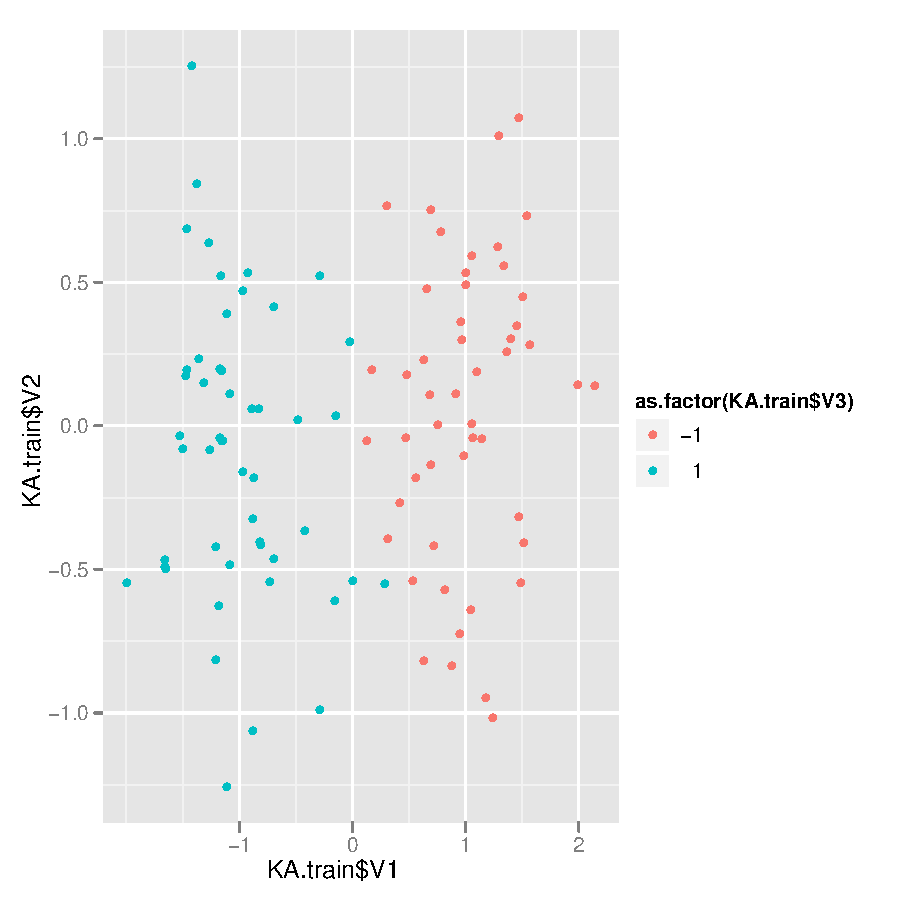
\includegraphics{Victor-loadKnoll}
Some random built-in R functions.
\begin{Schunk}
\begin{Sinput}
> require(MASS)
> require(klaR)
> covarA<-cov(cbind(KA.train$V1,KA.train$V2)) #covar for A. 
> ldaa<-lda(as.factor(V3) ~ ., data = KA.train)
> predA<-which(predict(ldaa,KA.test)$posterior[,2]>0.5) #indices where class==1
> sum(KA.test$V3[predA]==1)/length(which(KA.test$V3==1)) #accuracy=98%
\end{Sinput}
\begin{Soutput}
[1] 0.98
\end{Soutput}
\begin{Sinput}
> partimat(as.factor(V3)~.,data=KA.train,method="lda")
> ldab<-lda(as.factor(V3) ~ ., data = KB.train)
> predB<-which(predict(ldab,KB.test)$posterior[,2]>0.5) #indices where class==1
> sum(KB.test$V3[predB]==1)/length(which(KB.test$V3==1)) #accuracy=58% Hey, it's better than half.
\end{Sinput}
\begin{Soutput}
[1] 0.58
\end{Soutput}
\begin{Sinput}
> partimat(as.factor(V3)~.,data=KB.train,method="lda")
> ldac<-lda(as.factor(V3) ~ ., data = KC.train)
> predC<-which(predict(ldac,KC.test)$posterior[,2]>0.5) #indices where class==1
> sum(KC.test$V3[predC]==1)/length(which(KC.test$V3==1)) #accuracy=98%
\end{Sinput}
\begin{Soutput}
[1] 0.98
\end{Soutput}
\begin{Sinput}
> sum(KC.test$V3[predC]==-1)/length(which(KC.test$V3==1)) #accuracy=98%
\end{Sinput}
\begin{Soutput}
[1] 0.04
\end{Soutput}
\begin{Sinput}
> partimat(as.factor(V3)~.,data=KC.train,method="lda")
\end{Sinput}
\end{Schunk}
Fucking K-nearest neighbour. Implementing this seems easy enough: http://www.lkozma.net/knn2.pdf
http://www.scholarpedia.org/article/K-nearest_neighbor
\begin{Schunk}
\begin{Sinput}
> knn<-function(test,metric,train,k){
+   
+   if (metric=='euclidian'){
+     distance<-function(x,y){
+       return( sqrt((x[1]-y[1])^2+(x[2]-y[2])^2) )
+     }
+   }
+   
+   if (metric=='alternative'){
+     distance<-function(x,y){
+       M=matrix(c(100,0,0,1),2,2)
+       return(norm(M%*%x-M%*%y)) #f'real?
+     }
+   }
+   trainMat<-as.matrix(cbind(train$V1,train$V2))
+   d<-vector()
+   class<-vector()
+   i=1
+   while(i<=nrow(trainMat)) {
+     d<-append(d,(distance(x=trainMat[i,],y=test[c(1,2)])))
+     class<-append(class,train[i,]$V3)
+     i=i+1
+   }
+   map<-data.frame(cbind(d,class))
+   map<-map[order(map$d),]
+   
+   if(sum(map$class[1:k])>0){
+     return(1)
+   }
+   else{
+     return(-1)
+   }
+   
+ }
> knn(test=KA.test[9,],metric='euclidian',train=KA.train,k=3)
\end{Sinput}
\begin{Soutput}
[1] -1
\end{Soutput}
\begin{Sinput}
> knn(test=KA.test[9,],metric='alternative',train=KA.train,k=3)